%%
%% The first command in your LaTeX source must be the \documentclass command.
%% nonacm option turns off ACM stuff like copyright notice and such
\documentclass[sigplan,screen,nonacm]{acmart}

%%
%% \BibTeX command to typeset BibTeX logo in the docs
\AtBeginDocument{%
  \providecommand\BibTeX{{%
    \normalfont B\kern-0.5em{\scshape i\kern-0.25em b}\kern-0.8em\TeX}}}

% painint TODOs red    
\newcommand\TODO[1]{\textcolor{red}{\emph{TODO #1}}}

% for line break inside table cells
% t c or b for desired vertical alignment
\newcommand{\specialcell}[2][t]{%
  \begin{tabular}[#1]{@{}l@{}}#2\end{tabular}}

\usepackage[]{algorithm2e}
\usepackage{algorithmic}

%% end of the preamble, start of the body of the document source.
\begin{document}

%%
%% The "title" command has an optional parameter,
%% allowing the author to define a "short title" to be used in page headers.
\title[Hair Simulation]{Simulation of Curly Hair}
\subtitle{5th semester Project Laboratory report}

%%
%% The "author" command and its associated commands are used to define
%% the authors and their affiliations.
%% Of note is the shared affiliation of the first two authors, and the
%% "authornote" and "authornotemark" commands
%% used to denote shared contribution to the research.
\author{Barnabás Börcsök}
% \authornote{BSc student}
\email{borcsok.barnabas@simonyi.bme.hu}
\affiliation{%
  \institution{Budapest University of Technology and Economics}
  \city{}
  \country{}
}

\author{Dr. Szécsi László}
\email{Advisor}
\affiliation{%
    \institution{Budapest University of Technology and Economics}
    \city{}
    \country{}
    \department[0]{Computer Graphics Group}
    \department[1]{Department of Control Engineering and Information Technology}
}


%%
%% By default, the full list of authors will be used in the page
%% headers. Often, this list is too long, and will overlap
%% other information printed in the page headers. This command allows
%% the author to define a more concise list
%% of authors' names for this purpose.
% \renewcommand{\shortauthors}{Trovato and Tobin, et al.}

%%
%% The abstract is a short summary of the work to be presented in the
%% article.
\begin{abstract}
    A self-assessment of the 5th semester Project Laboratory
    Project is presented in this article. My goal was to achieve hair simulation
    of acceptable quality both in terms of look and performance. Multiple
    approaches were considered before arriving at a Position Based Dynamics
    based solution. The simulation was implemented in C++ with the Open Graphics
    Library (OpenGL \footnote{\url{http://www.opengl.org}}). 
\end{abstract}

%%%
%%% The code below is generated by the tool at http://dl.acm.org/ccs.cfm.
%%% Please copy and paste the code instead of the example below.
%%%
\begin{CCSXML}
<ccs2012>
<concept>
<concept_id>10010147.10010371.10010352.10010379</concept_id>
<concept_desc>Computing methodologies~Physical simulation</concept_desc>
<concept_significance>300</concept_significance>
</concept>
</ccs2012>
\end{CCSXML}

\ccsdesc[300]{Computing methodologies~Physical simulation}
%%
%% Keywords. The author(s) should pick words that accurately describe
%% the work being presented. Separate the keywords with commas.
\keywords{hair simulation, position based dynamics, OpenGL}

%% A "teaser" image appears between the author and affiliation
%% information and the body of the document, and typically spans the
%% page.
\begin{teaserfigure}
  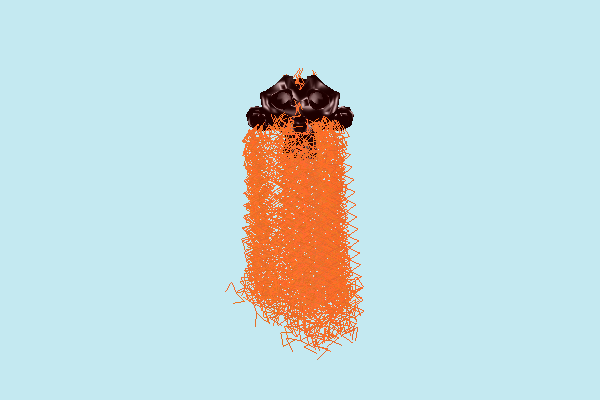
\includegraphics[width=\textwidth]{teaser.png}
  \caption{The achieved visual look}
  \Description{Using 400 hair pieces, with 25 particles on each piece of hair.}
  \label{fig:teaser}
\end{teaserfigure}

%%
%% This command processes the author and affiliation and title
%% information and builds the first part of the formatted document.
\maketitle
\renewcommand{\shortauthors}{Barnabás Börcsök}


\section{Introduction}
In the 5th semester of their undergrad studies, BSc students from Budapest
University of Tehchnology and Economics embark on their first journey of
scientific research. I was always interested in and fascinated by computer 
graphics, it came naturally to choose a subject in this area. As I had little
 hands-on experience in this field, a long time had to be dedicated
to research and trying out different simulation methods.

The first of this paper reflects this, giving an overview of considered methods,
and other possible routes that could have been taken to implement hair
simulation.


The implementation and all of the code mentioned is avaiable at
\url{http://git.sch.bme.hu/bobarna/brave-2}.

\section{Overview of considered methods}

There were mainly three methods considered, two of them being substantially
different:


\subsection{Mass Spring System}
The whole idea of doing hair simulation as my project laboratory came after
reading \citet{PixarPaper}. They outline a method for the artistic simulation of
curly hair for use in their film production. The method was featured in the 2012
movie Brave.

This approach models the hair as a chain of particles with given mass, each
connected via springs. This results in a mass-spring system, which is then
modelled by considering well-known physics formula's such as Newton's second law
of motion $F=m*a$, and Hooke's Law, which states that the force $F$
needed to extend or compress a spring by some distance $x$ scales linearly with
respect to that distance. The paper by \citet{PixarPaper} created an elaborate
system of springs, with additional core springs making the simulation stable
and resulting in the desired look and feel.

The main characteristic of this approach is that a Mass Spring System deals with
forces, and tries to stay true to the laws of physics. It accounts for internal 
and external forces from which accelerations are computed based on Newton's 
second law of motion. A time integration method is then used to update the
velocities and finally the positions of the particles. This will not be the case
with Position Based Dynamics.
\subsection{Position Based Dynamics (PBD)}

The paper by \citet{MullerPBD} presents an approach that omits the velocity as
well as the force layer of the then-present popular approaches for simulation
methods of dynamic systems in computer graphics.

Position Based Dynamics (PBD) -- as its name suggests -- works with the position
of particles. A big advantage of such a system lies in its controllability, and
the easy reducability of overshooting problems present in force based systems.
Another favorable aspect is that PBD methods are generally easier with the maths
and somewhat easier to implement in terms of the needed mathematical and
physical background needed to grasp its inner workings. In addition, -- as it
works directly with the position of particles -- collision constraints can be
handled easily and penetrations can be resolved completely by projecting points
onto the penetrated surface. Although such measures can only be applied on the
expanse of physical accuracy, position based dynamics being only a ``good
enough'' approximation of how objects behave in real life.

Chapter 2 of the paper by \citet{UmenhofferSimulation} builds on the
\citet{MullerPBD} paper and gives a concise overview of the position based
dynamics method, and goes on to show the type of constraints that can be applied
to control to behaviour of such a system -- which is present in both papers.


\subsection{Follow-the-Leader (FTL)}
The Dynamic Follow-the-Leader (FTL) method outlined in \citet{FTLHair} focuses
on the fast simulation of hair and fur on animated characters. The sheer number
of computation needed for simulating thousands of hair strands, each consisting
of numerous particles presents a big challenge. Also, as each strand is
inextensible, it is not trivial to come up with an algorithm that does its job
in feasible time. 

As it will be covered later in this article, the already introduced PBD method
needs multiple iterations per frame in order to keep the system from stretching
and becoming unstable. The FTL method by \citet{FTLHair} presents a method that
takes only a single iteration through the particles of each hair strand per
frame to achieve the desired results.

As this sounds fascinating, and cuts the computation time needed substantially,
in the early stages of my project, I implemented the FTL method alongside PBD.
It \textit{works}, and is fast, although due to the iteration count being one,
when greater forces are being applied to the system, a substantial amount of
stretching was introduced to the system. As it seemed in comparison that the
``basic'' PBD method yielded the same -- or even more accurate -- results, and
it was feasible to allow myself to use multiple iterations per frame, I did
not further investigate if there could have been improvements made to my
implementation to eliminate the stretching in the presence of greater forces.


\section{Simulation of a Single Hair Strand}

\subsection{A Particle}

We model an $S$ hair strand as a chain of $P$ particles and a set of $C$
constraints. Each particle $p \in [1,\ldots,N]$ has three atributes: mass ($m_p$), position
($\boldsymbol{x_p}$) and velocity ($\boldsymbol{v_p}$). 

A constraint $c \in [1,\ldots,C]$ with cardinality $n_c$ is a function $C_c
: \mathbb{R} ^{3n_c} \mapsto \mathbb{R}$. It operates on a set of indices $\{i_1,\ldots
i_{n_c}\}, i_k \in [1,...,P]$. The constraint funtion also has a stiffnes
parameter $k_c \in [0...1]$ and a type of either \emph{equality} or
\emph{inequality}.

Constraint $c$ with type \emph{equality} is satisfied if
$C_c(\boldsymbol{x}_{p_1},\ldots, \boldsymbol{x}_{p_{n_j}})=0$. If its type is
\emph{inequality}, then it is satisfied if $C_c(\boldsymbol{x}_{p_1}, \ldots,
\boldsymbol{x}_{p_{n_c}}) \geq 0$. The stiffness parameter $k_c$ defines the
strength of the constraint in a range from zero to one.

Given these notations, the algorithm works in the following way:

\begin{algorithm}
    \caption{pseudo code for the PBD simulation}
    \label{alg:pseudoPBD}
    \begin{algorithmic}
        \IF {$i \geq maxval$}
            \STATE asd
        \ENDIF
    \end{algorithmic}
\end{algorithm}

\begin{verbatim}
    class Particle {
        vec3 pos;
        vec3 tmp;
        float w;
        vec3 v;
        vec3 color;
    }
\end{verbatim}

\section{Putting Hair on the Head}



\section{Results}
The implementation is available at \url{git.sch.bme.hu/bobarna/brave-2}. The
program is able to handle up to around 500 individual hair strands, each
consisting of around 30 particles in real time. With the implemented OBJ reader,
it is possible to achieve diverse visual results in no time. The 

An example result shown in figure \TODO{include figure}, and can be seen in the
supplementary videos \TODO{Google Drive (?) link with the videos}.

An 8-minute-video was made to supplement this writing. It is accessible at
\TODO{link to 8-minute video}

\section{Conclusion}
After investigating and trying out multiple methods to simulate hair, we arrived
at the Position Based Dynamics (PBD) method. An overview of the PBD method, and
an introduction to the constraint types used in our implementation was given.
An implementation was made in C++ and OpenGL, which easily simulates the hair
strands in real time, although the limit of the real-time nature can easily be
surpassed when adding around a thousand strands each with more than 30
particles.

\section{Future Work}
As this was part only of a semester-long Project Laboratory course, a great deal
of time was dedicated in the early stages of the project to investigate and
explore the subject area. This left only a sub-optimal time for implementing all
desired aspects of the simulation.

\subsection{Hair-hair collisions}
As it is computationally extensive to simulate each particle colliding with all
of the other particles, a particle density field could be used. One such method
of grouping hair particles and their corresponding velocities into a 3D voxel
grid is outlined in the \citet{PixarVolumetricHair} paper, which was also
utilized in the \citet{FTLHair} paper for handling hair-hair collisions.

\subsection{Refinement and proper customizability of the propagation of hair
strands on the head object.} 
A drawable texture map is considered for the ability to tell the simulation
where to put the hair strands on the surface of the head.

\subsection{Better customizability}
In the current implementation there is no way to properly customize the look and
feel of the hair without accessing the source code. A possible improvement could
be to read material and texture data for the hair from the OBJ file. Another
huge improvement could be to set the constraints in real time, giving the user
much better control of the hair. Other properties, such as length of the hair
segments and color of the hair could be set as well.

\subsection{Halton sequence for randomizing hair positions}
In the current implementation, a standard C++ random number generator is
utilized. Utilizing a low-discrepancy number sequence for randomizing hair
strand positions would be an improvement.

\subsection{Rendering}
This semester left no time to try out different methods for rendering and
visualizing the hair. The current implementation connects the individual
particles with GL\_LINES, resulting in a sub-optimal visual experience. Offline
(e.g. ray-tracing) methods could utilize the current simulation method. 
The paper by \citet{RappRealTime} discusses the real-time aspect of hair
rendering in great detail, supplemented with a broad discussion on different
parts of the (OpenGL) rendering pipeline that could be utilized.

\subsection{Moving to the GPU}
The current implementation runs solely on the CPU. A big leap forward would be
the utilization of the GPU. Compute shaders for computations are considered. The
paper by \citet{UmenhofferSimulation} discusses a parametrization of the
different constraint solves, although as they work on the same dataset, some
computation problems are present during the parellelization of the
problem.

Tesselation and geometry shaders could be utilized for the rendering and display
of the particles, resulting in a far better image with the same simulation
method and properties.

%%
%% The acknowledgments section is defined using the "acks" environment
%% (and NOT an unnumbered section). This ensures the proper
%% identification of the section in the article metadata, and the
%% consistent spelling of the heading.
\begin{acks}
    To Dr. László Szécsi, associate professor at the Computer Graphics Group
    (Department of Control Engineering and Information Technology), whom I had
    the chance to consult with during the semester.
\end{acks}

%%
%% The next two lines define the bibliography style to be used, and
%% the bibliography file.
\bibliographystyle{ACM-Reference-Format}
\bibliography{references}

%%
%% If your work has an appendix, this is the place to put it.
\appendix

\section{Supplementary development}

\subsection{OBJ Reader}

An OBJ reader utility was implemented as part of the project. As the OBJ file
format \footnote{\url{http://paulbourke.net/dataformats/obj/}} describes a wide range
of properties for objects. The present OBJ reader handles only the subset of
these describtion options needed for the project. Lines containing other type of
object descriptions were ignored, resulting in a successful file read if
possible.

\begin{table}[htb]
    \caption{Supported OBJ Data Types} 
    \label{tab:objdatatypes}
    % \begin{minipage}{\columnwidth}
        \begin{center}
            \begin{tabular}{ll}
                % \toprule
                Type of data & Format\\
                Comment & \# \verb|comment|\\
                Geometric vertex data & \verb|v x y z| \\
                Texture coordinates & \verb|vt u v| \\
                Vertex normals &\verb|vn i j k| \\
                Triangular faces &
                \specialcell{\texttt{f v1/vt1/vn1
                v2/vt2/vn2}\\\multicolumn{1}{r}{\texttt{... v3/vt3/vn3}}}\\
                % \bottomrule
            \end{tabular}
        \end{center}
    % \end{minipage}
\end{table}

\newcommand{\vFootNote}{\footnote{The obj file format allows for a w coordinate
(also called the weight) for describing rational curves and surfaces. The
default value of \textit{w} is 1.0. My implementation handles only the
assignment of \textit{x}, \textit{y} and \textit{z} values.}}

\newcommand{\vtFootNote}{\footnote{The obj file format allows for 3D texture
coordinates as well, but this implementation handles only 2D texture
coordinates.}}

\newcommand{\fFootNote}{\footnote{The obj file format allows for face
definitions far beyond only triangles, although this implementation handles only
face definitions of the above format.}}

\begin{itemize}
    \item ``\verb|v x y z|'' defines a vertex with position (x, y, z).\vFootNote 
    \item ``\verb|vt u v|'' defines a 2D texture coordinate with position (u,
        v).\vtFootNote 
    \item ``\verb|vn i j k|'' specifies a normal vector with components i, j and
        k.  
    \item ``\verb|f v1/vt1/vn1 v2/vt2/vn2 v3/vt3/vn3|'' Specifies a face with the
        given indices. For the first vertex, the \textit{v1}st previously
        defined vertex position is used, the \textit{vt1}st texture coordinate
        and \textit{vn1}st normal vector is used.\fFootNote
\end{itemize}


\subsection{Recording the simulation on-the-fly}
A recording utility was made to work in tandem with the application. In essence,
the rendered images are written into \texttt{bmp} or \texttt{png} files if the
capturing is on. In the
implementation\footnote{\url{https://git.sch.bme.hu/bobarna/brave-2}}, toggling
the capturing is mapped to the \texttt{C} key.


For handling the export of the rendered image into files, the
stb\_image\_write.h\footnote{\url{https://github.com/nothings/stb/blob/master/stb\_image\_write.h}}
single-file public domain library was used. 


The program outputs the image files in the \texttt{renders} folder at 24 FPS,
with the naming convention renderXXXX[.bmp/.png], where XXXX is the number of
the frame with left-padded zeroes.


After the image files are written, the user can start the
\texttt{make\_video.sh} script to assemble the \texttt{output.mp4} and delete
all the rendered frames. This script uses the free and open-sorce ffmpeg command
line utility\footnote{\url{https://ffmpeg.org/}}


\end{document}
\endinput
%%
%% End of file `documentation.tex'.
